% # COPYRIGHT:
%
% Copyright (C) 2011 Jeremiah Mahler <jmmahler@gmail.com>.
% Permission is granted to copy, distribute and/or modify this document
% under the terms of the GNU Free Documentation License, Version 1.3
% or any later version published by the Free Software Foundation;
% with no Invariant Sections, no Front-Cover Texts, and no Back-Cover Texts.
% A copy of the license is included in the file "fdl-1.3.txt".
%
\documentclass[12pt]{article}
%\usepackage{mslapa}
\usepackage{hyperref}
\usepackage{amsmath}
\usepackage{graphicx}
\usepackage{ulem}
\usepackage{vmargin}
\usepackage{tabularx}
\usepackage{sectsty}
\usepackage{pbox}
\usepackage{bigstrut}
\usepackage{enumerate}
\usepackage{parskip} % add spaces between paragraphs
\input kvmacros % Karnaugh Maps and Veitch charts
%\usepackage{cleveref}
\setpapersize{USletter}
%\setpapersize{A4}
%\setmarginsrb{<leftmargin>}{<topmargin>}{<rightmargin>}{<bottommargin>}
% {<headheight>}{<headsep>}{<footheight>}{<footskip>}
%\setmarginsrb{1.25in}{1.0in}{1.0in}{1.0in}{0in}{0.25in}{0in}{0.20in}
\setmarginsrb{1.0in}{1.0in}{1.0in}{1.0in}{0in}{0.25in}{0in}{0.20in}
\sectionfont{\normalsize}
\subsectionfont{\normalsize}
% configure \bigstrut size
% This configures spacing above and below rows in a tabularx.
%\renewcommand{\bigstrutjot}{6pt}
\renewcommand{\bigstrutjot}{2.0\jot}
\setlength{\parindent}{0in}
\raggedright
\begin{document}

% {{{ Cover Page
\centerline{\bf EECE 144}
\centerline{\bf Fall 2011}
\centerline{\bf}
\centerline{\bf Lab Report \#7}
\centerline{\bf Section 4}
\centerline{\bf 10/19/2011}
% signature area
\begin{center}
\begin{tabularx}{\textwidth}[b]{X l l}
Submitted by: Marvanee Johnson & & \\
Signature & Printed Name & Date \\
\hline
\multicolumn{1}{|X|}{} & \multicolumn{1}{|l|}{\bigstrut \bf Marvanee Johnson} & \multicolumn{1}{|l|}{\bf Oct 19, 2011} \\
\hline
\multicolumn{1}{|X|}{} & \multicolumn{1}{|l|}{\bigstrut \bf Jeremiah Mahler} & \multicolumn{1}{|l|}{\bf Oct 19, 2011} \\
\hline
\end{tabularx}
\end{center}
% }}}

\section{Description/Objectives}
% description
The purpose of this lab is to find the min SOP expressions of equations $J$ \& $K$
(Equation \ref{eq:Jcsop} and \ref{eq:Kcsop}) using a minimal amount of gates
and to build a circut combining the two equations using only two input gates.

\begin{align}
J(w, x, y, z) &= \sum m(1,3,9,11,12,13,14,15) \label{eq:Jcsop} \\
K(w, x, y, z) &= \sum m(0,1,3,12,14) \label{eq:Kcsop}
\end{align}
\section{Procedure}
\label{sec:procedure}
The first step in accomplishing this task was to create separate
Karnaugh Map for expressions $J$ \& $K$ in order to find the min SOPs of the
equations and to determine the number of gates needed to implement each
equation separately. The next step was to jointly optimize the two equations
through the use Karnaugh Maps to produce a circuit using the minimum number
of gates.
Lastly, we used the Truth table (Table \ref{tbl:tt}) in order to test
and verify the functionality of the circuit.

\begin{table}[tbp]
\begin{center}
\begin{tabular}{lr}
\begin{tabular}[t]{r|cccc|c|c}
Index&$w$&$x$&$y$&$z$&$J$&$K$\\
\hline
0 &0&0&0&0 &0 &1\\
1 &0&0&0&1 &1 &1\\
2 &0&0&1&0 &0 &0\\
3 &0&0&1&1 &1 &1\\
4 &0&1&0&0 &0 &0\\
5 &0&1&0&1 &0 &0\\
6 &0&1&1&0 &0 &0\\
7 &0&1&1&1 &0 &0\\
8 &1&0&0&0 &0 &0\\
9 &1&0&0&1 &1 &0\\
10 &1&0&1&0 &0 &0\\
11 &1&0&1&1 &1 &0\\
12 &1&1&0&0 &1 &1\\
13 &1&1&0&1 &1 &0\\
14 &1&1&1&0 &1 &1\\
15 &1&1&1&1 &1 &0\\
\end{tabular}
\end{tabular}
\end{center}
\caption{Truth table of functions $J$ and $K$.}
\label{tbl:tt}
\end{table}

The minimal SOP expression for $J$ was found by the use of a Karnaugh Map
(Figure \ref{fig:Jmap}) resulting in equation \ref{eq:Jsop}.

\begin{equation}
J = w x + x' z \label{eq:Jsop}
\end{equation}
\begin{figure}[!hbt]
\begin{center}
\karnaughmap{4}{$J(w,x,y,z)$:}{wxyz}{0101000001011111}{}
\end{center}
\caption{Karnaugh map of function $J$ (Equation \ref{eq:Jcsop}).}
\label{fig:Jmap}
\end{figure}

The minimal SOP expression for $K$ was found by the use of a Karnaugh Map
(Figure \ref{fig:Kmap}) resulting in equation \ref{eq:Ksop}.

\begin{figure}[tbp]
\begin{center}
\karnaughmap{4}{$K(w,x,y,z)$:}{wxyz}{1101000000001010}{}
\end{center}
\caption{Karnaugh map of function $K$ (Equation \ref{eq:Kcsop}).}
\label{fig:Kmap}
\end{figure}
\begin{equation}
K = w'x'y' + w'x'z + wxz' \label{eq:Ksop}
\end{equation}

A gifted mind of electronics can probably deduce the number of
gates and gate inputs from the expressions alone.
But here we appeal to the not so brilliant of us by using
circuit diagrams to clearly elucidate the metrics we
are seeking.

\samepage
Referring to the circuit for $J$ in Figure \ref{fig:Jminsop-01} we
can see that there are 2 AND gates, 1 OR gate, and 1 NOT gate.
And there are 4 inputs to the AND gates, 2 inputs to the OR gate,
and 1 input to the NOT gate.

\begin{figure}[tbp]
\center
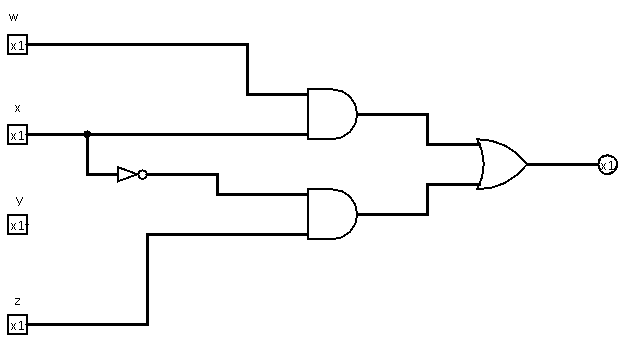
\includegraphics[scale=0.5]{Jminsop-01}
\caption{Circuit diagram of the minimal SOP solution of $J$.}
\label{fig:Jminsop-01}
\end{figure}

Referring to the circuit for $K$ in Figure \ref{fig:Kminsop-01} we
can see that there are 3 AND gates, 1 OR gate and 4 NOT gates.
And there are 9 inputs to the AND gates, 3 inputs to the OR gate,
and 4 inputs to the NOT gates.

\begin{figure}[tbp]
\center
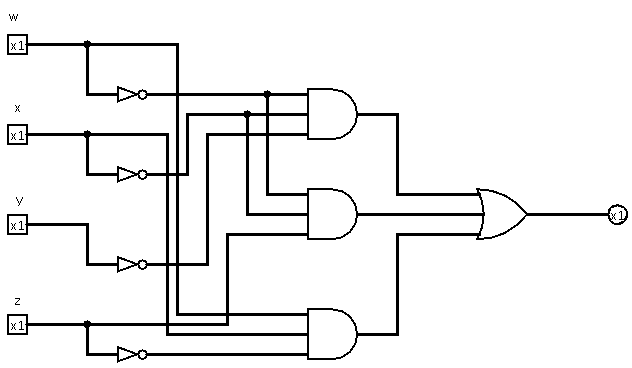
\includegraphics[scale=0.5]{Kminsop-01}
\caption{Circuit diagram of the minimal SOP solution of $K$.}
\label{fig:Kminsop-01}
\end{figure}

When limited to two gates the previous solution for $J$ is the
same.
For $K$ the circuit must be modified as shown in Figure \ref{fig:Kminsop-02}.
This results in 4 NOT gates, 6 AND gates and 2 OR gates.
And there are 4 inputs to the NOT gates, 12 inputs to the AND gates
and 4 inputs to the OR gates.

\begin{figure}[tbp]
\center
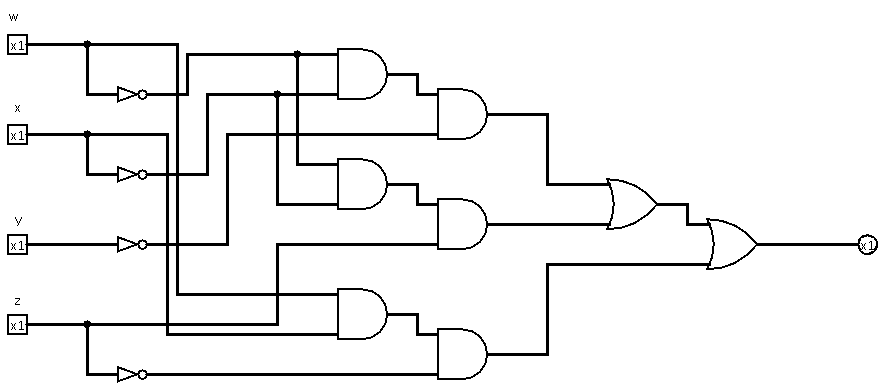
\includegraphics[scale=0.5]{Kminsop-02}
\caption{Circuit diagram of the minimal SOP solution of $K$ when limited to two input gates.}
\label{fig:Kminsop-02}
\end{figure}
\clearpage

A jointly optimized solution of $J$ and $K$ is created by combining shared
terms used by both SOP expressions of $J$ and $K$ as show in
Figure \ref{fig:JKjointkmap}.
And Equation \ref{eq:JKjoint} is the resulting expressions.

\begin{align}
J &= w'x'z + wxz' + wz \notag \\
K &= w'x'z + wxz' + w'x'y' \label{eq:JKjoint}
\end{align}
\begin{figure}[tbp]
\center
%\karnaughmap{4}{$J(w,x,y,z)$:}{wxyz}{0101000001011111}{}
%\karnaughmap{4}{$K(w,x,y,z)$:}{wxyz}{1101000000001010}{}
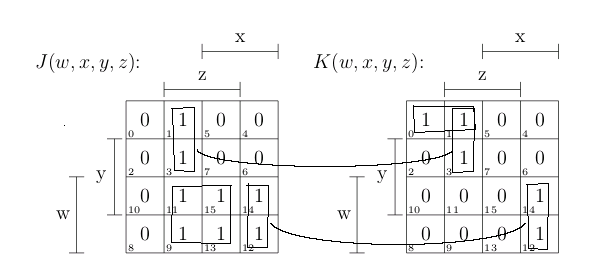
\includegraphics[scale=0.60]{JKkmap-01}
\caption{Jointly optimized Karnaugh maps for $J$ and $K$.}
\label{fig:JKjointkmap}
\end{figure}

And the circuit diagram of the jointly optimized solution is given
in Figure \ref{fig:JKjointcircuit}.
It can be seen that there are 4 NOT gates, 7 AND gates and 4 OR gates.
There are 4 NOT gate inputs, 14 AND gate inputs, and 8 OR gate inputs.

\begin{figure}[tbp]
\center
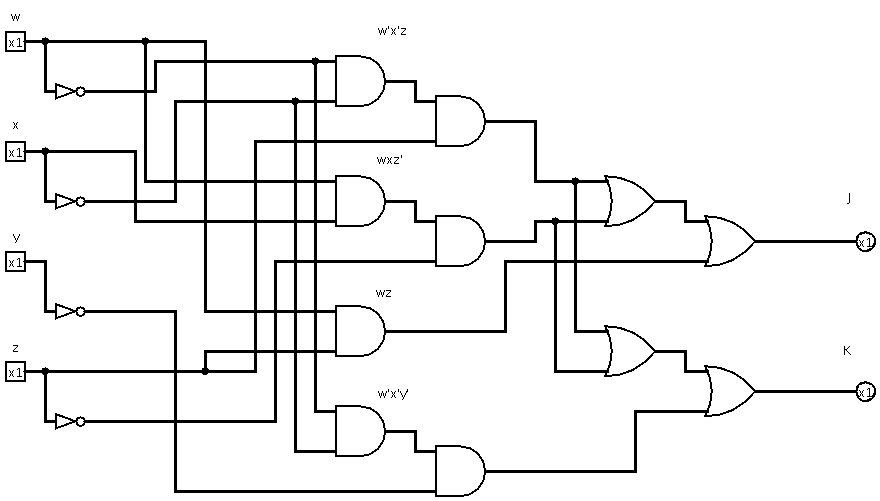
\includegraphics[scale=0.5]{JKjoint-01}
\caption{Circuit diagram of the jointly optimized solution of $J$ and $K$ when limited to two input gates.}
\label{fig:JKjointcircuit}
\end{figure}

Finally this jointly optimized solution (Figure \ref{fig:JKjointcircuit}
can be implemented using the 74HC04(NOT), 74HC08(AND),
and 74HC32(OR) ICs.
Pull down resistors (1k ohms works well) must be used on the switch inputs.
The current through the LED outputs should be limited using a 270 ohm resistor.
And if the LED outputs do not work try reversing their direction (remember
they behave like diodes).

\clearpage

\section{Observations}

The jointly optimized solution (Figure \ref{fig:JKjointcircuit}) of functions
$J$ and $K$ reproduced the expected truth table values (Table \ref{tbl:tt}).

The jointly optimized solution did reduce the number of gates
albeit slightly.
It can be seen from Table \ref{tbl:counts} that implementing
$J$ and $K$ independently resulted in 16 gates and 27 inputs.
Implementing these jointly resulted in 15 gates and 26 inputs,
a savings of 1 gate and 1 input.

\begin{table}[!htb]
\center
\begin{tabular}{cc}
\begin{tabular}{lll}
\multicolumn{3}{c}{\bf{$J$ by itself}} \\
gate type & \# gates & \# inputs\\
\hline
AND & 2 & 4\\
OR & 1 & 2\\
NOT & 1 & 1 \\
\hline
\bf{TOTAL} & 4 & 7
\end{tabular}
&
\begin{tabular}{lll}
\multicolumn{3}{c}{\bf{$J$ and $K$ independently}} \\
gate type & \# gates & \# inputs\\
\hline
AND & 8 & 16 \\
OR & 3 & 6 \\
NOT & 5 & 5 \\
\hline
\bf{TOTAL} & 16 & 27
\end{tabular}
\\
\\
\begin{tabular}{lll}
\multicolumn{3}{c}{\bf{$K$ by itself, 2 input gates}} \\
gate type & \# gates & \# inputs\\
\hline
AND & 6 & 12 \\
OR & 2 & 4 \\
NOT & 4 & 4 \\
\hline
\bf{TOTAL} & 12 & 20
\end{tabular}
&
\begin{tabular}{lll}
\multicolumn{3}{c}{\bf{$J$ and $K$ jointly}} \\
gate type & \# gates & \# inputs\\
\hline
AND & 7 & 14 \\
OR & 4 & 8 \\
NOT & 4 & 4 \\
\hline
\bf{TOTAL} & 15 & 26
\end{tabular}
\end{tabular} % outer formatting table
\caption{Metrics of gate and input counts for various configurations
of $J$ and $K$.}
\label{tbl:counts}
\end{table}

\section{Conclusion}

The lab was a success in demonstrating that shared hardware can be used
to implement separate expressions and still produce the desired outcome.

% flush all the figures
%\clearpage
% Uncomment these if you have references,
%\pagebreak
%\renewcommand*{\refname}{\vspace{-8mm}}
%\section{References}
%%\bibliographystyle{plain}
%%\bibliographystyle{mslapa}
%\bibliographystyle{ieeetr}
%\bibliography{../references}
% Appendix (if needed)

\end{document}

% vim:foldmethod=marker
